
   \documentclass{standalone}
   \usepackage{tikz}
   %\usetikzlibrary{positioning,shapes}
   \usepackage{pgfplots}
   \begin{document}
   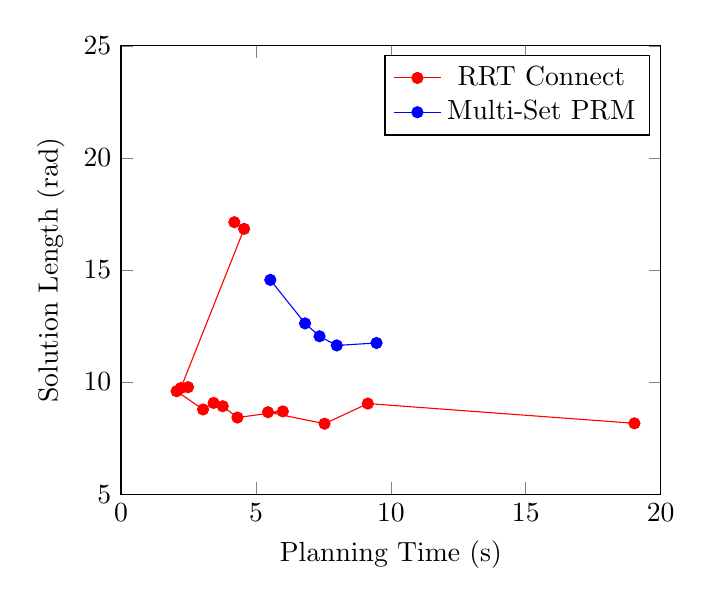
\begin{tikzpicture}
   
   \begin{axis}[
      xlabel=Planning Time (s),
      ylabel=Solution Length (rad),
      ylabel near ticks,
      xlabel near ticks,
      xmin=0,xmax=20,
      ymin=5,ymax=25]
   
   \addplot[mark=*,red] plot coordinates {
     (19.0274559021,8.15935852501)
  (9.14634549617,9.03977101653)
  (7.54299542903,8.14138799804)
  (5.44797422886,8.65535253002)
  (5.99811706543,8.69111056932)
  (4.31411030292,8.41667616907)
  (3.77034747601,8.92238622474)
  (3.43184010983,9.06853080166)
  (3.04022064209,8.77742643549)
  (2.05956606865,9.59148400767)
  (2.48428049087,9.77166550607)
  (2.21680300236,9.7299063202)
  (4.56119611263,16.8339112477)
  (4.19993259907,17.1317529022)

   };
   \addlegendentry{RRT Connect}
   
   \addplot[mark=*,blue] plot coordinates {
     (9.46978783607,11.7433568343)
  (7.99695899487,11.6339708521)
  (7.3566380024,12.0419836982)
  (6.82064850331,12.6166565966)
  (5.53297576904,14.5578704775)

   };
   \addlegendentry{Multi-Set PRM}
   
   
   \end{axis}
   
   \end{tikzpicture}
   \end{document}
   
